% Metódy inžinierskej práce

\documentclass[10pt,twoside,slovak,a4paper]{article}

\usepackage[slovak]{babel}
%\usepackage[T1]{fontenc}
\usepackage[IL2]{fontenc} % lepšia sadzba písmena Ľ než v T1
\usepackage[utf8]{inputenc}
\usepackage{graphicx}
\usepackage{url} % príkaz \url na formátovanie URL
\usepackage{hyperref} % odkazy v texte budú aktívne (pri niektorých triedach dokumentov spôsobuje posun textu)
\usepackage{graphicx}
\graphicspath{ {./obrazky/} }
\usepackage{cite}
%\usepackage{times}

\pagestyle{headings}

\title{Vyhľadávanie najlepšieho ťahu v šachu\thanks{Semestrálny projekt v predmete Metódy inžinierskej práce, ak. rok 2023/24, vedenie: Vladimír Mlynarovič}} % meno a priezvisko vyučujúceho na cvičeniach

\author{Martin Kubiš\\[2pt]
	{\small Slovenská technická univerzita v Bratislave}\\
	{\small Fakulta informatiky a informačných technológií}\\
	{\small \texttt{xkubis@stuba.sk}}
	}

\date{\small 30. september 2023} % upravte



\begin{document}

\maketitle

\begin{abstract}
Šach je strategická stolová hra, ktorá sa skladá z šachovnice o rozmeroch 8x8 a 6 typov figúriek vo dvoch farbách. Aj keď sa na prvý pohľad zdá ako jednoduchá hra, neprestáva trápiť mozgy hráčov jak začiatočníkov, tak profesionálov. Od 50. rokov 20 storočia, kedy sa vyvinul prvý šachový robot, sa vývoj nezastavil a počítače už sú na míle ďaleko pred ľudskými hráčmi. Cielom článku je priblíženie čitateľovi metódy a techniky šachových algoritmov, ich optimalizácia, takisto aj porovnanie medzi klasickými šachovými algoritmami a algoritmami obohatené o umelú inteligenciu a ako vyhľadávajú najefektívnejší možný ťah.
\ldots
\end{abstract}



\section{Úvod}
Šach je jednou z najstarších a najpopulárnejších hier, ktorá sa v priebehu storočí stala symbolom intelektu, stratégie a výzvy pre ľudský mozog. 

Hranie šachu si vyžaduje veľa zručností, strategické myslenie, plánovanie určitých ťahov, schopnosť predvídať a dokonca byť nepredvídateľný. Aby sa hráči zlepšili, či už na profesionálnej alebo amatérskej úrovni, musia rozvíjať svoje zručnosti a znalosti o šachových algoritmoch a stratégiach, ktoré sú kľúčom k úspechu v tejto komplexnej hre.

Tento článok sa zameria na šachové algoritmy, aké sú stratégie určené na zlepšenie schopností hráča, pochopenie hry a vyhladanie čo najlepších možných žahov na prekonanie súpera. Šachové algoritmy sú rozhodujúce pre šachové programy, ktoré sú čoraz výkonnejšie a každým dňom umožňujú posúvať hranice toho, čo sme si mysleli, že je možné v oblasti rýchlosti a presnosti ťahov.

V tomto článku preskúmame históriu šachových algoritmov, pričom sa zameriame na najdôležitejšie algoritmy ako sú minimax algoritmus s alfa-beta pruningom, monte carlo tree search algoritmus, alebo využitie deep learningu, neurálnych sietí a umelej inteligencie a poukážeme na využitie týchto algoritmov v modernom šachovom svete. Ďalej sa budeme venovať technickým výzvam spojeným s vývojom šachových programov a ich schopnosťou hrať na úrovni šachových majstrov. 

Nakoniec sa dotkneme etických a filozofických otázok spojených s používaním šachových algoritmov a umelej inteligencie vo svete šachu.


\section{Minimax algoritmus} \label{minimax}
Minimax algoritmus je rozhodovací algoritmus používaný v hrách na určenie najlepšieho možného ťahu pre hráča v hre pre dvoch hráčov s nulovým súčtom, ako je napríklad šach alebo piškôrky. V hre s nulovým súčtom sú zisky jedného hráča presne vyvážené stratami druhého hráča, takže súčet ziskov a strát hráčov je vždy nula. 




\subsection{Princíp fungovania Minimax algoritmu} \label{principMinimax}
Minimax algoritmus funguje tak, že predpokladá, že obaja hráči budú hrať optimálne, a potom určí najlepší ťah pre hráča, ktorý práve robí ťah. 

Robí to tak, že zvažuje všetky možné ťahy, ktoré by hráč mohol urobiť, a potom hodnotí každý z týchto ťahov simulovaním zvyšku hry za predpokladu, že súper urobí svoj najlepší možný ťah. Algoritmus potom vyberie ťah, ktorý vedie k najlepšiemu výsledku pre hráča, za predpokladu, že súper ako odpoveď urobí svoj najlepší možný ťah.
\begin{figure}[h]
    \centering
    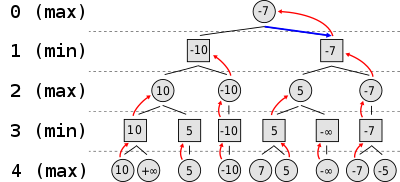
\includegraphics[width=\textwidth]{minimax}
    \caption{obr1: Jednoduchá ukážka minimax algoritmu}
    \label{obr1}
\end{figure}

\subsection{Výhody a obmedzenia Minimax algoritmu} \label {vyhodyMinimax}

Minimax algoritmus je výkonný a teoretický prístup k rozhodovaniu o hrách, ktorý poskytuje optimálne riešenia v zmysle teórie hier. Tento algoritmus má však niekoľko obmedzení. Prvým je jeho výpočtová náročnosť, najmä v hrách s veľkým rozhodovacím priestorom. Preto boli vyvinuté rôzne varianty a optimalizácie, ako napríklad:
\begin{itemize}
\item Alpha-Beta pruning
\item Otváracie ťahy (Openings)
\end{itemize}
Vďaka týmto optimalizáciam sa zníži počet vetví, cez ktoré musí algoritmus prejsť, taktiež sa vylepší celkový výkon algoritmu. 


Môže sa zdať, že problém vlastne nejestvuje\cite{Coplien:MPD}, ale bolo dokázané, že to tak nie je~\cite{Czarnecki:Staged, Czarnecki:Progress}. Napriek tomu, aj dnes na webe narazíme na všelijaké pochybné názory\cite{PLP-Framework}. Dôležité veci možno \emph{zdôrazniť kurzívou}.


\section{Alpha-Beta pruning} \label{alpha-beta}
V praxi väčšina AI šachových robotov používa optimalizovanú verziu minimax algoritmu známeho ako alfa-beta pruning algoritmus. Základnou myšlienkou alfa-beta pruningu je zníženie počtu vetiev, ktoré je potrebné hodnotiť „prerezávaním“(pruningom) konárov, ktoré istotne nepovedú k lepšiemu výsledku ako tie, ktoré už boli hodnotené. 

To sa dosiahne použitím dvoch hodnôt, alfa a beta, na sledovanie najlepšieho výsledku, ktorý bol doteraz zistený pre maximalizujúceho hráča (alfa) a najlepšieho výsledku, ktorý bol doteraz nájdený pre minimalizujúceho hráča (beta)

\subsection{Princíp fungovania alpha-beta pruningu} \label{principAlpha-beta}
Algoritmus funguje tak, že rekurzívne skúma strom hry a vyhodnocuje každý možný pohyb a výsledok pomocou algoritmu minimax. Pri skúmaní každej vetvy stromu aktualizuje hodnoty alfa a beta na základe najlepšieho výsledku, ktorý bol doteraz nájdený. 

Ak nájde vetvu, v ktorej je výsledok pre minimalizujúceho hráča (beta) horší ako aktuálny najlepší výsledok pre maximalizujúceho hráča (alfa), prereže túto vetvu a prestane ju vyhodnocovať, pretože minimalizujúci hráč by tento ťah nikdy nezvolil. 

Algoritmus postupuje rekurzívne nahor po strome, pričom neustále aktualizuje hodnoty alfa a beta, kým nevyhodnotí všetky možné pohyby a výsledky, alebo kým neoreže všetky vetvy, ktoré sú zaručene horšie ako aktuálny najlepší výsledok.
\begin{figure}[h]
    \centering
    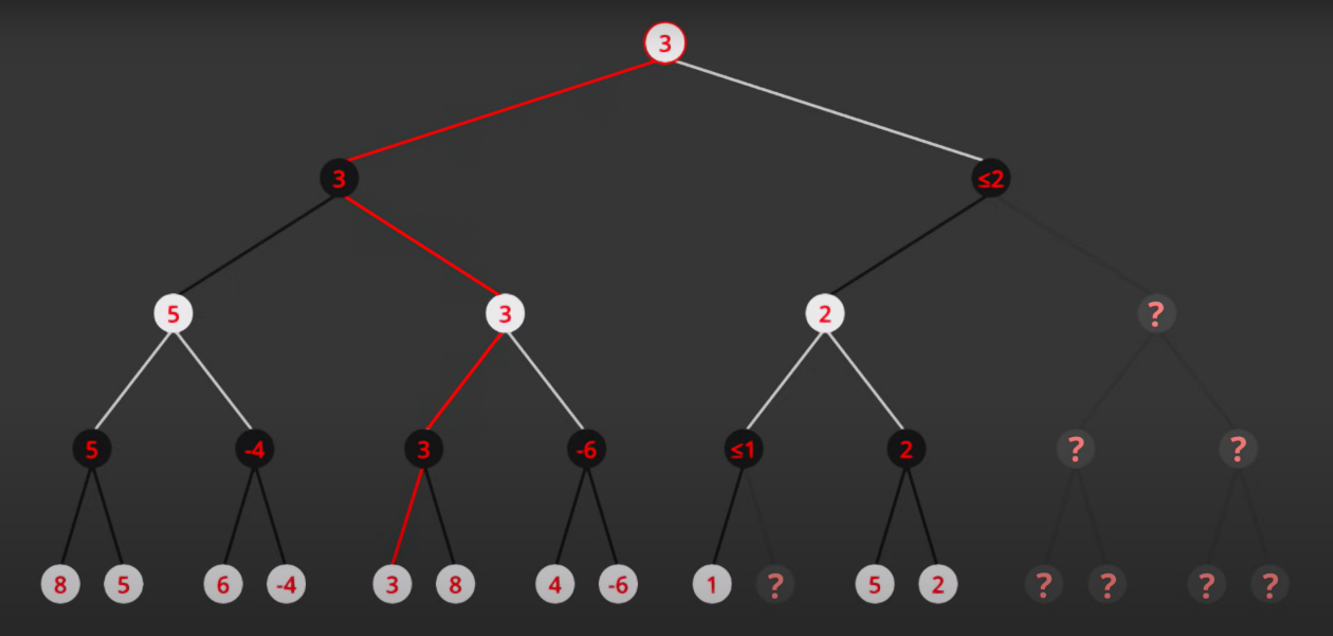
\includegraphics[width=\textwidth]{alpha-beta}
    \caption{obr2: ukážka alpha-beta pruningu}
    \label{obr2}
\end{figure}


\section{Monte Carlo Tree Search} \label{MonteCarlo}
Monte Carlo Tree Search (MCTS) je inovatívny a výkonný algoritmus v oblasti umelej inteligencie a teórie hier, ktorý bol využitý na rôzne stolové hry, ako je napríklad Go a šach. Tento algoritmus výrazne prekonáva tradičné techniky vyhľadávania v stromovom priestore, čím umožňuje získať vysokokvalitné výsledky v hrách s veľkými rozhodovacími priestormi.

\section{Princíp fungovania MCTS} \label{PrincipMTCS}
MCTS sa líši od predchádzajúcich algoritmov Minimax tým, že neprehľadáva celý stromový priestor. Namiesto toho sa používa metóda vzorkovania, pri ktorej sa ťahy vyberajú a simulujú až do konca hry, aby sa získal odhad aktuálneho stavu hry. Opakuje tento proces niekoľkokrát a na základe získaných hodnôt sa rozhodne, ktorý ťah je najlepší. V MCTS existujú štyri základné fázy: výber, šírenie, simulácia a spätné šírenie.
\begin{enumerate}
	\item výber (Selection)
	\item šírenie (Expansion)
	\item simulácia (Simulation)
	\item spätné šírenie (Backpropagation)
\end{enumerate}

\begin{figure}[h]
    \centering
    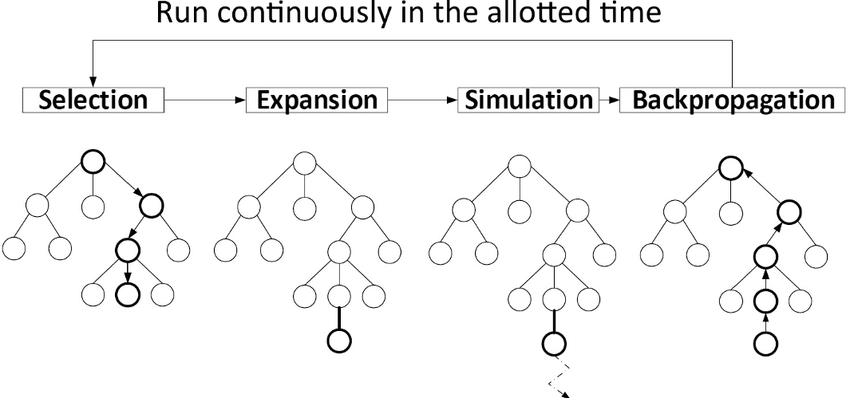
\includegraphics[width=\textwidth]{MCTS}
    \caption{obr3: ukážka fungovania MCTS}
    \label{obr2}
\end{figure}
\paragraph{Veľmi dôležitá poznámka.}
Niekedy je potrebné nadpisom označiť odsek. Text pokračuje hneď za nadpisom.



\section{DeepLearning, Neural networks} \label{DeepNeural}







\section{Záver} \label{zaver} % prípadne iný variant názvu



%\acknowledgement{Ak niekomu chcete poďakovať\ldots}


% týmto sa generuje zoznam literatúry z obsahu súboru literatura.bib podľa toho, na čo sa v článku odkazujete
\bibliography{literatura}
\bibliographystyle{plain} % prípadne alpha, abbrv alebo hociktorý iný
\end{document}
